To study the structure of IRS 63, intensity profiles were extracted along the minor axis in both \SI and debiased polarized intensity at each wavelength. The locations of the slices are shown in Figure \ref{fig: slice-along-minor}.




% ------------------------------------------------
\begin{figure}[htbp]
  \centering
  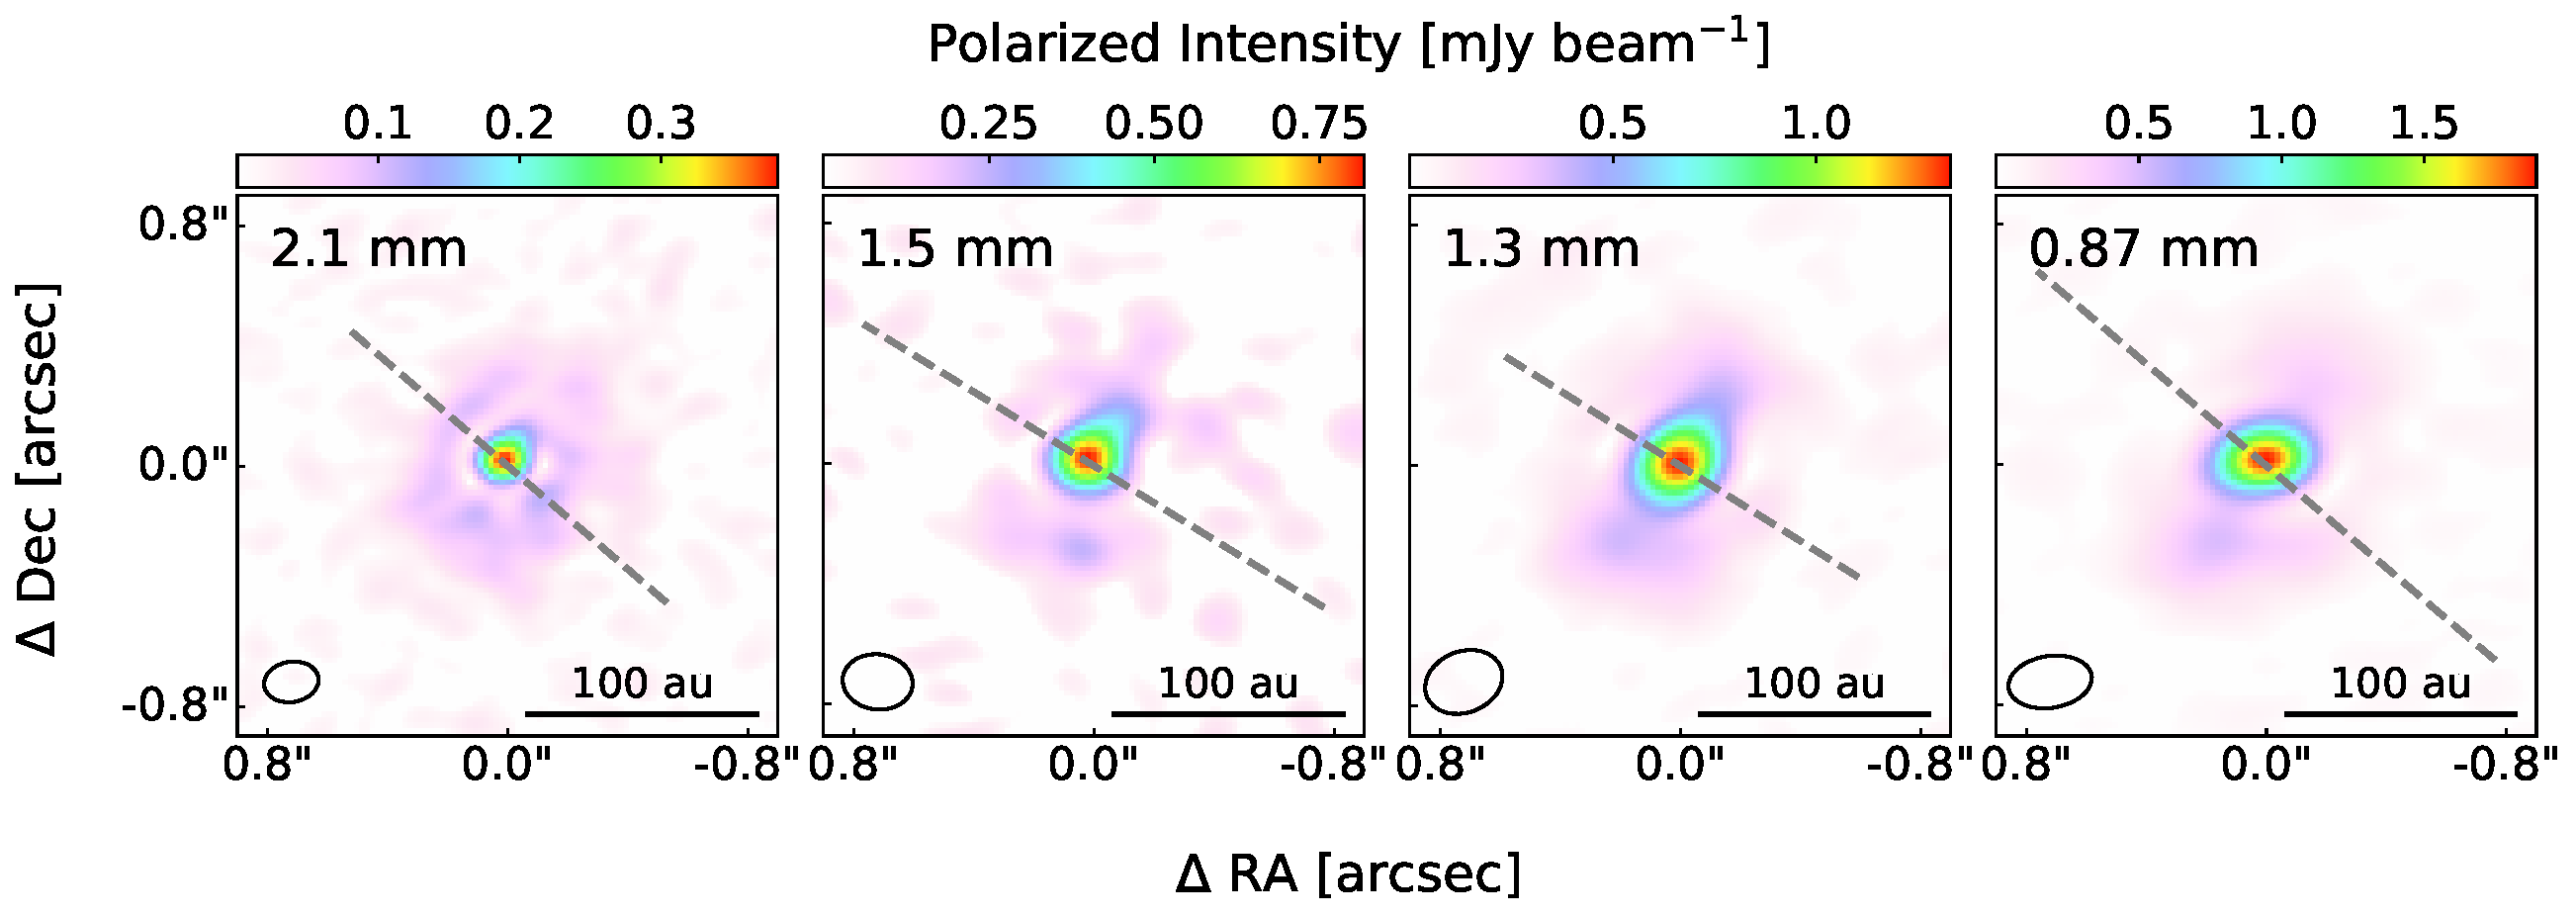
\includegraphics[width=0.99\textwidth]{WRITEUP_AND_IMAGES/IMAGES/WRITEUP/Slices/MinorAxisSliceGrid_robust_minus1_Delta.pdf}
  \caption{Locations of the minor-axis slices extracted from the images at each wavelength. The same slice was used for both \SI and debiased polarized intensity.}
  \label{fig: slice-along-minor}
\end{figure}
% ------------------------------------------------




The slices in \SI and polarized intensity for each wavelength are presented in Figure \ref{fig: slices_grid}. The synthesized beam for each wavelength is overplotted for comparison. The beam is plotted as a one-dimensional Gaussian, with a standard deviation calculated from the beam full width at half maximum (FWHM) along the minor axis using:
\begin{equation}
    \sigma = \frac{\text{FWHM}}{2\sqrt{2 \ln{2}}}.
    \label{eq: FWHM_to_sigma}
\end{equation}
\noindent The Gaussian was normalized to 1 and scaled by the peak intensity of each slice. 
% \noindent The standard deviations are used to calculate the Gaussian shape at each offset using:
% \begin{equation}
%     \text{Beam(offset)} = \exp{\left(-\frac{\text{offset}^2}{2\sigma^2}\right)},
% \end{equation}
% \noindent which was then normalized to 1 and scaled by the maximum value of the slice. 




The \SI profiles (top row of Figure \ref{fig: slices_grid}) show a single peak at the centre of the disk at all four wavelengths. This is expected, as the density of the disk increases towards the central star, resulting in stronger emission from the inner disk. However, in the debiased polarized intensity profiles (bottom row of Figure \ref{fig: slices_grid}), we do not see the same trend. The profiles are consistently offset from the centre position at all four wavelengths. Relative to the synthesized beam, the offset is not well resolved. However, the offset is observed across all four wavelengths indicates that it is real. 




An offset in polarized intensity relative to total intensity could be a geometric effect due to the disk being both puffy and inclined. \cite{Yang} showed that optically thick disks that are both flared and inclined should have brighter polarized intensities on the near side of the disk.  This difference is due to forward scattering (from the near side) being favoured over back scattering (from the far side).  Thus, Figure \ref{fig: slices_grid} demonstrates that IRS 63 is likely flared, meaning its vertical scale height increases with radius (Figure \ref{fig: dust-grain-growth-schematic}). Unfortunately, the angular resolution of the data is insufficient to further model the polarization intensity and constrain the flaring.









\begin{figure}[htbp]
  \centering
  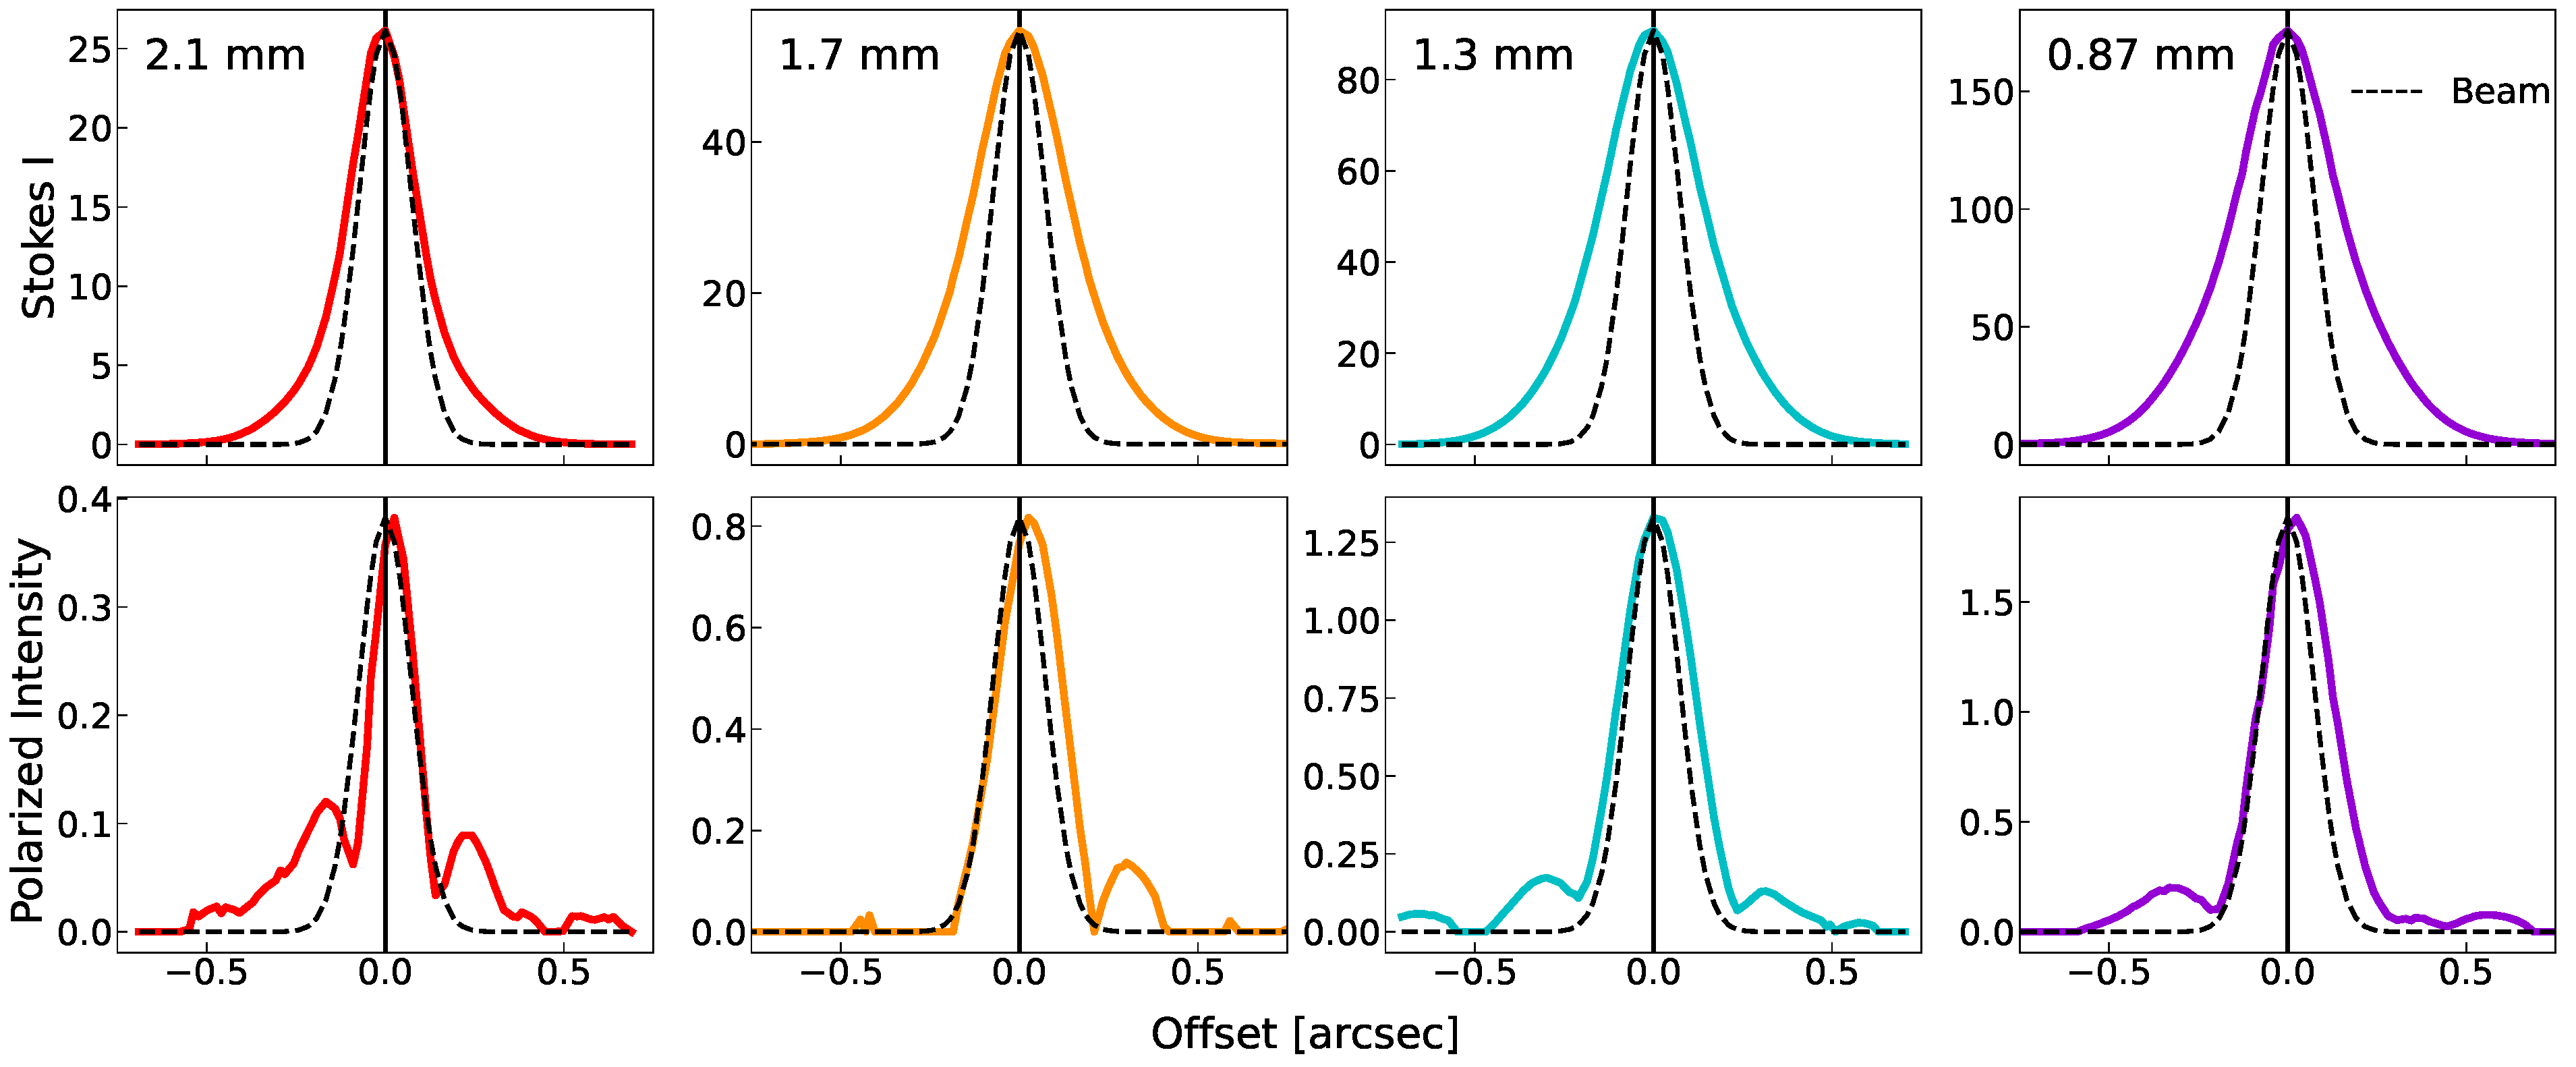
\includegraphics[width=0.99\textwidth]{WRITEUP_AND_IMAGES/IMAGES/WRITEUP/Slices/MW_slices_GRID.pdf}
  \caption{Plot of (top) \SI and (bottom) polarized intensity offset as a function of the offset from the centre position of the disk, both in units of mJy beam$^{-1}$. The centre position is shown as a solid black line, with the corresponding values found in Table \ref{tab: source_info}. The slices used for these profiles are shown in Figure \ref{fig: slice-along-minor}. }
  \label{fig: slices_grid}
\end{figure}





% Separate plots
% -------------------------------------------------
% \begin{figure*}[h]
%   \centering
%   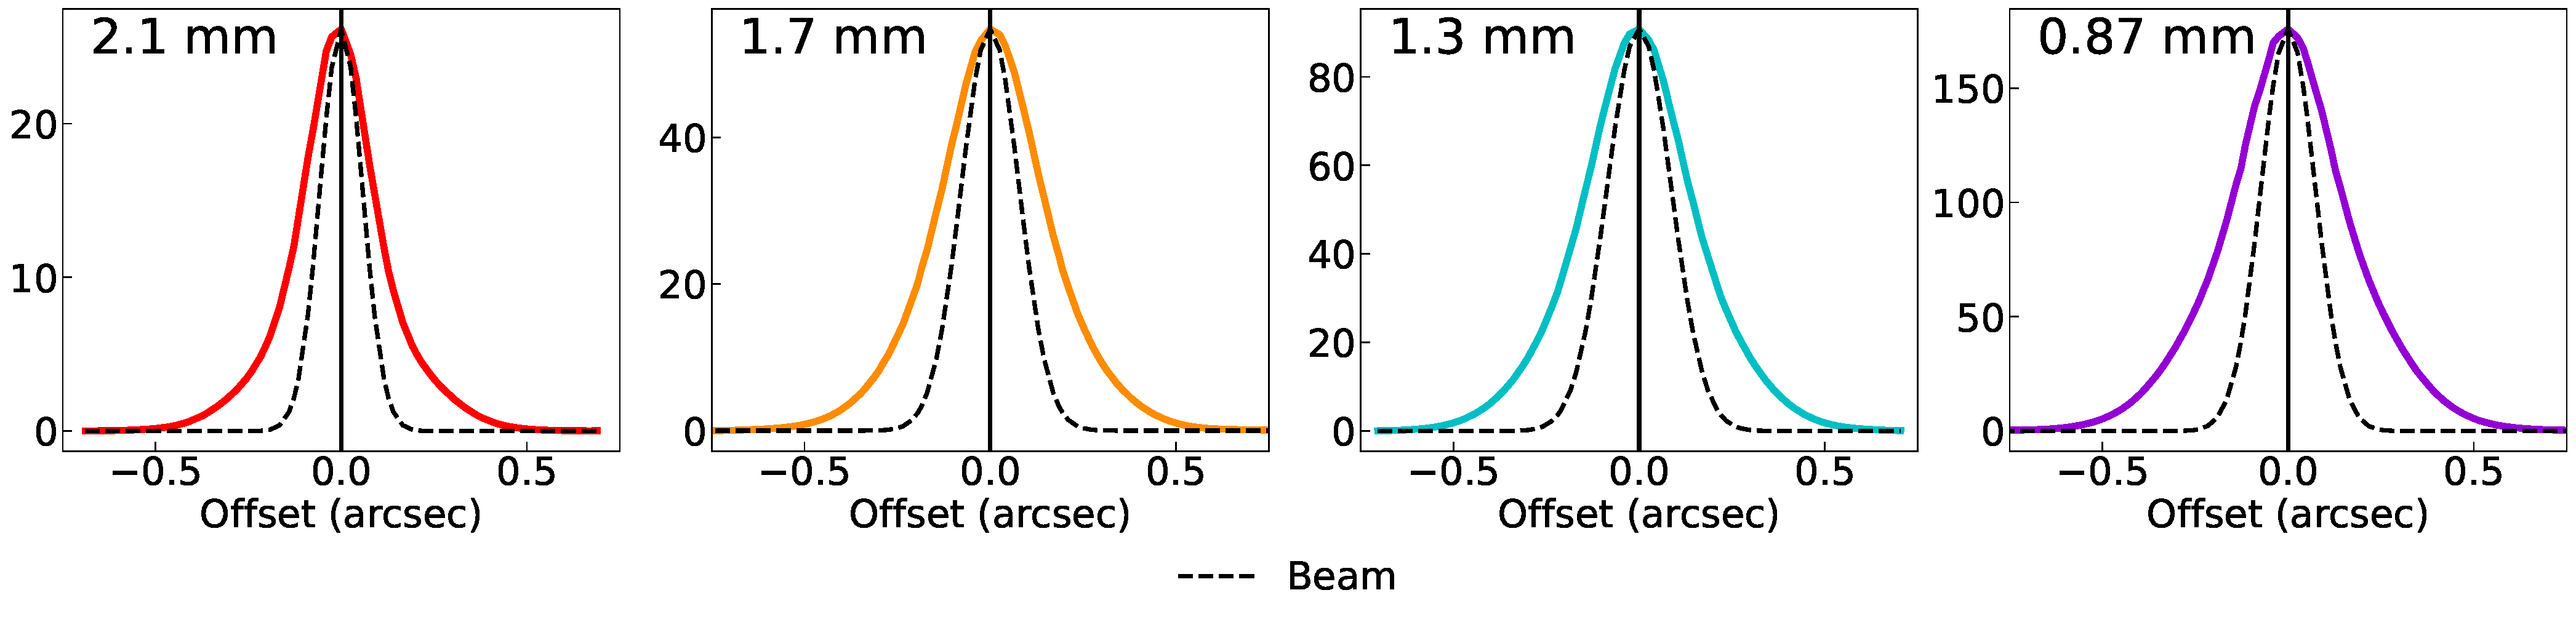
\includegraphics[width=1.1\textwidth]{../IMAGES/WRITEUP/Slices/MW_slices_StokesI_with_beam.pdf}
%   \caption{Plot of \SI versus offset from the centre position of the disk. The centre position values can be found in Figure \ref{tab: source_info}, and the slices are shown in Figure \ref{fig: slice-along-minor}. A solid black line is shown at an offset of 0. \add{Comment about beam}. Units are mJy per beam. }
%   \label{fig: slices_StokesI}
% \end{figure*}
% -------------------------------------------------
% \begin{figure*}[h]
%   \centering
%   
\includegraphics[width=1.1\textwidth]{W../IMAGES/WRITEUP/Slices/MW_slices_StokesI.pdf}
%   \caption{Plot of Stokes I in mJy versus offset from the centre position of the disk. The centre position values can be found in Figure \ref{tab: source_info}, and the slices are shown in Figure \ref{fig: slice-along-minor}. A solid black line is shown at an offset of 0. }
%   \label{fig: slices_StokesI}
% \end{figure*}
% -------------------------------------------------

% \begin{figure*}[h]
%   \centering
%   \includegraphics[width=1.1\textwidth]IMAGES/WRITEUP{WRITEUP_AND_IMAGES//Slices/MW_slices_POLI.pdf}
%   \caption{Same as Figure \ref{fig: slices_StokesI}, but for POLI.}
%   \label{fig: slices_POLI}
% \end{figure*}
% -------------------------------------------------
% \begin{figure*}[h]
%   \centering
%   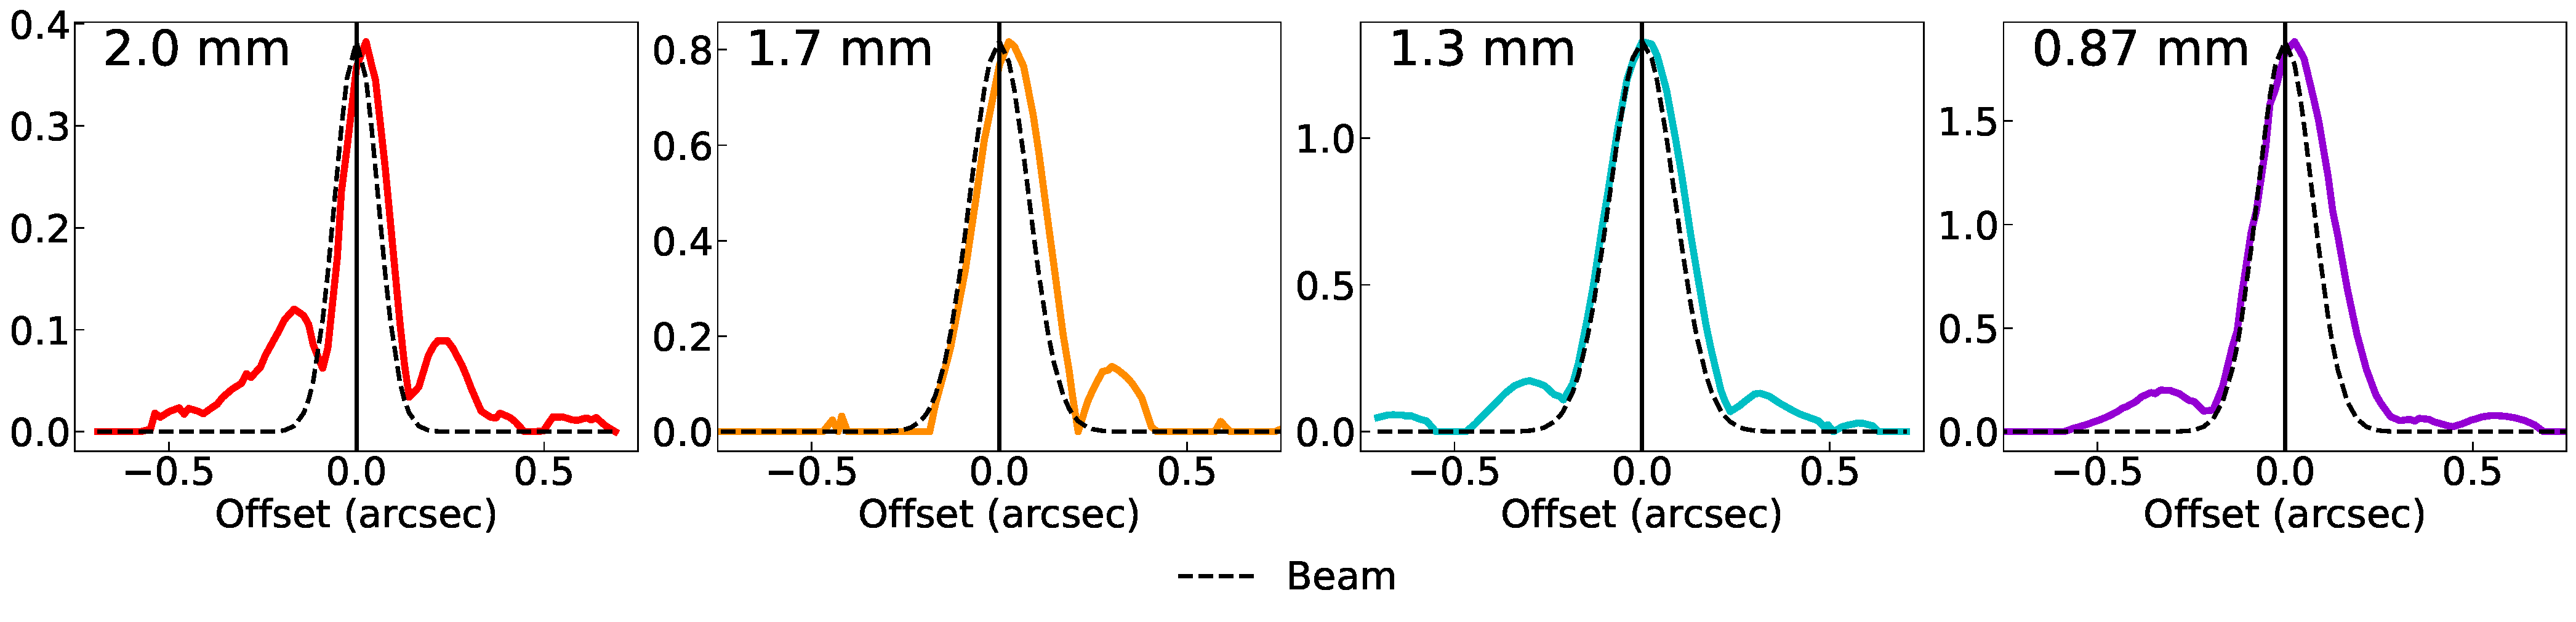
\includegraphics[width=1.1\textwidth]{../IMAGES/WRITEUP/Slices/MW_slices_POLI_with_beam.pdf}
%   \caption{Same as Figure \ref{fig: slices_StokesI}, but for polarized intensity.}
%   \label{fig: slices_POLI}
% \end{figure*}
% -------------------------------------------------

